\chapter{Experiments}
\section{Dropout Experiment}

\begin{figure}[H]
   \centering
   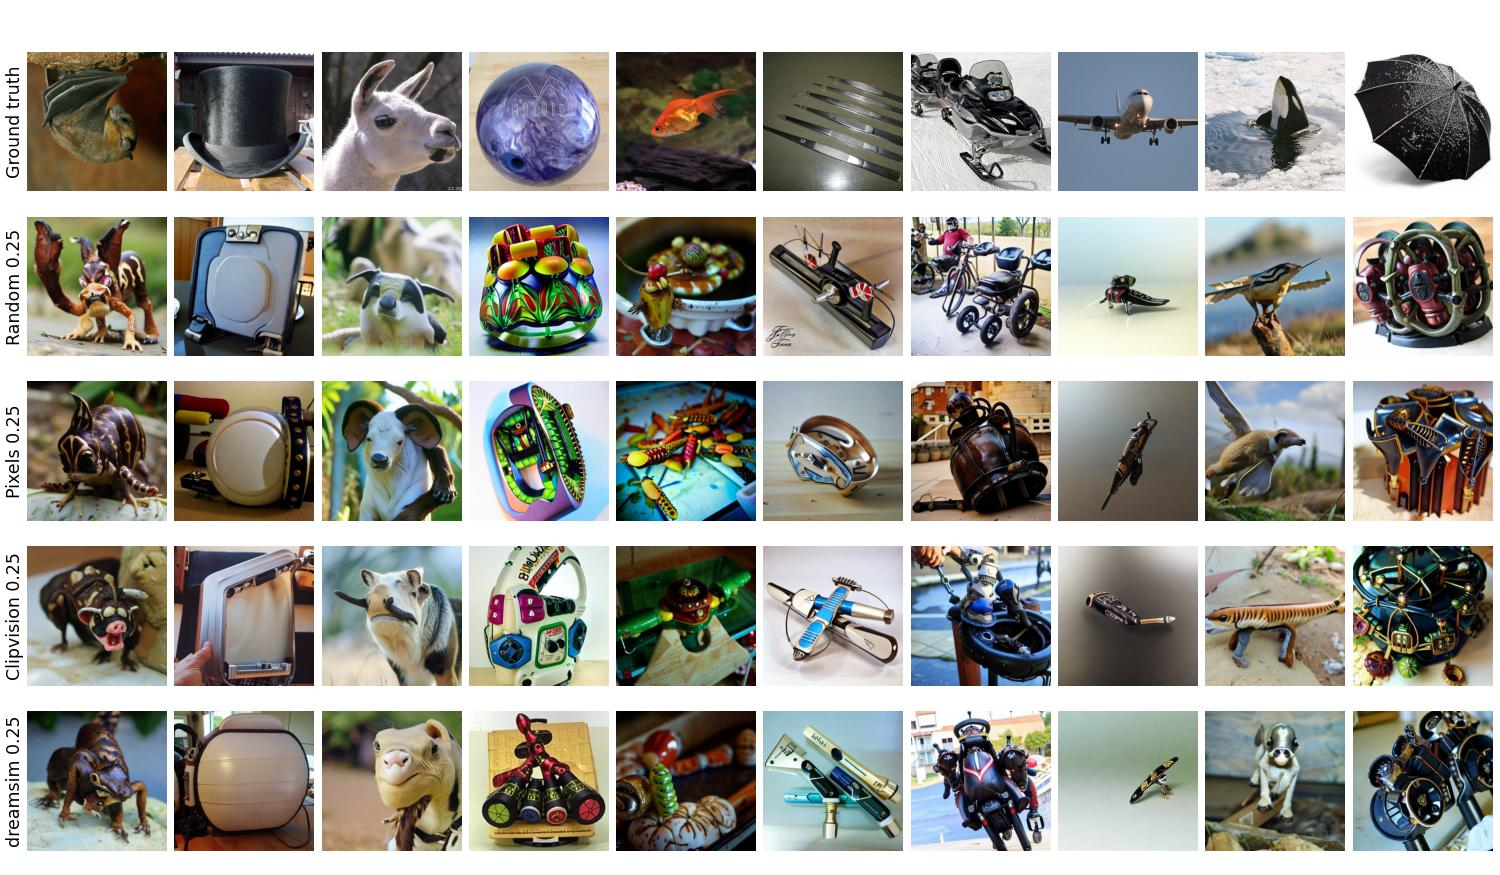
\includegraphics[width=1\textwidth]{plots/dropout_qual_eval_bd_test.JPEG}
   \caption[Experiment 1: Reconstructed images for Brain-Diffuser on natural test images]{Qualitative Results for different dropout strategies with the Brain-Diffuser on natural test images. The top row depicts the ground truth image. Each following row depicts the reconstruction where the translator was trained using the dropout strategy defined on the left side.}\label{fig:dropout_qual_eval_bd_test}
\end{figure}

\begin{figure}[H]
   \centering
   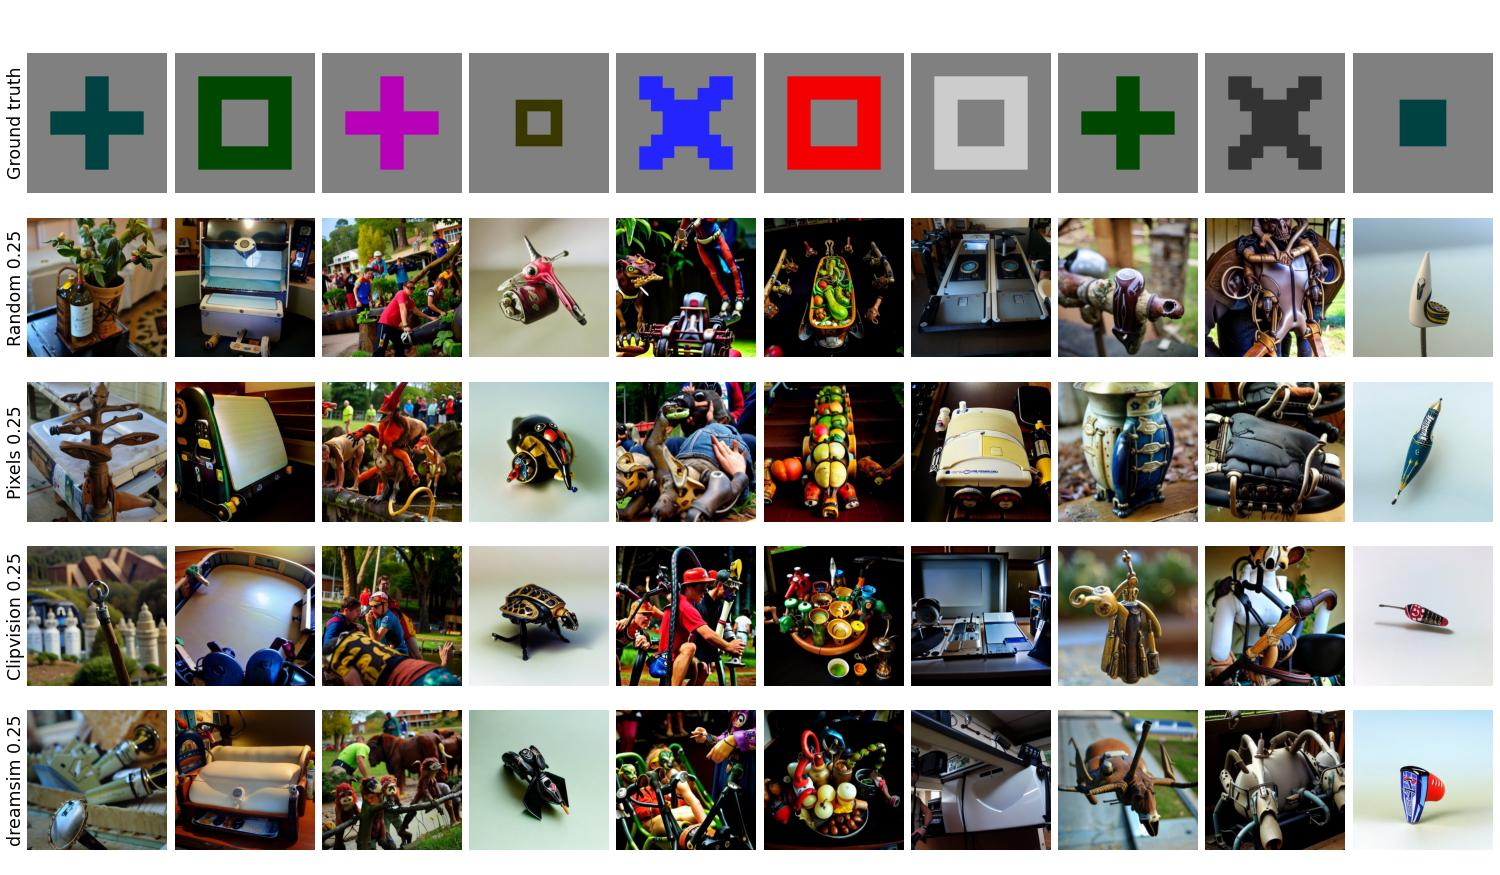
\includegraphics[width=1\textwidth]{plots/dropout_qual_eval_bd_art.JPEG}
   \caption[Experiment 1: Reconstructed images for Brain-Diffuser on artificial shapes]{Qualitative Results for different dropout strategies with the Brain-Diffuser on artificial shapes. The top row depicts the ground truth image. Each following row depicts the reconstruction where the translator was trained using the dropout strategy defined on the left side.}\label{fig:dropout_qual_eval_bd_art}
\end{figure}


\begin{figure}[H]
   \centering
   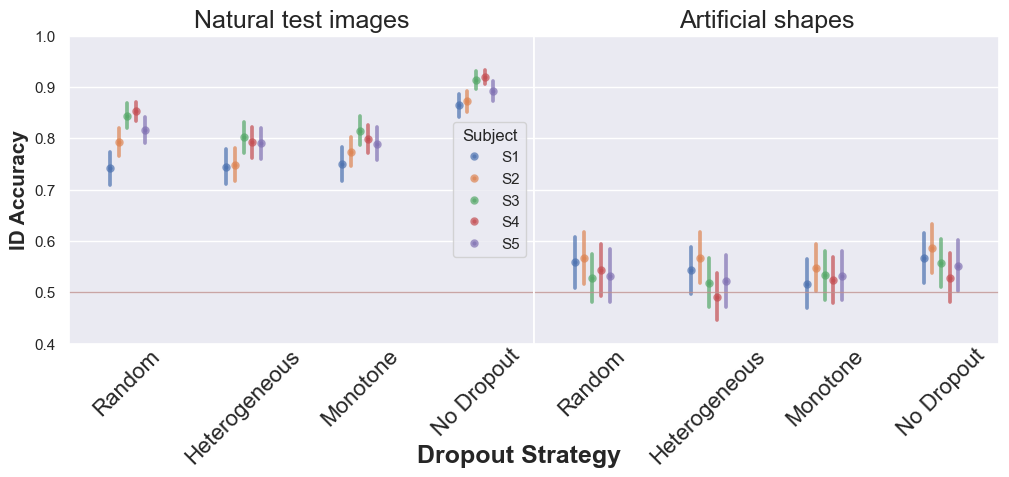
\includegraphics[width=1\textwidth]{plots/dropout_discussion_translator_id_acc_cliptext.png}
   \caption[CLIP Text translator Results for monotone vs.\ heterogeneous training images]{CLIP Text translator Results for monotone vs.\ heterogeneous training images. The identification accuracy of the CLIP Text translator is displayed for a different samples of the training data: a random subset, a heterogeneous subset, a monotone subset and the full training data. The results are shown for both the natural test images and the artificial shapes. The data is shown for each subject, the error bars are computed as the standard error across all test samples.}
   \label{fig:dropout_discussion_translator_id_acc_cliptext}
 \end{figure}
 
 \begin{figure}[H]
   \centering
   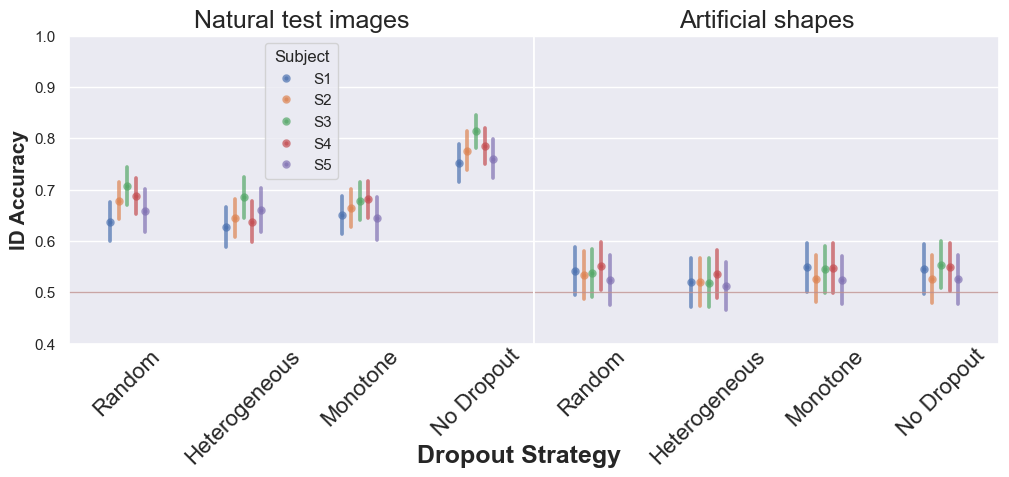
\includegraphics[width=1\textwidth]{plots/dropout_discussion_translator_id_acc_clipvision.png}
   \caption[CLIP Vision translator Results for monotone vs.\ heterogeneous training images]{CLIP Vision translator Results for monotone vs.\ heterogeneous training images. The identification accuracy of the CLIP Vision translator is displayed for a different samples of the training data: a random subset, a heterogeneous subset, a monotone subset and the full training data. The results are shown for both the natural test images and the artificial shapes. The data is shown for each subject, the error bars are computed as the standard error across all test samples.}\label{fig:dropout_discussion_translator_id_acc_clipvision}
 \end{figure}
 
 \begin{figure}[H]
   \centering
   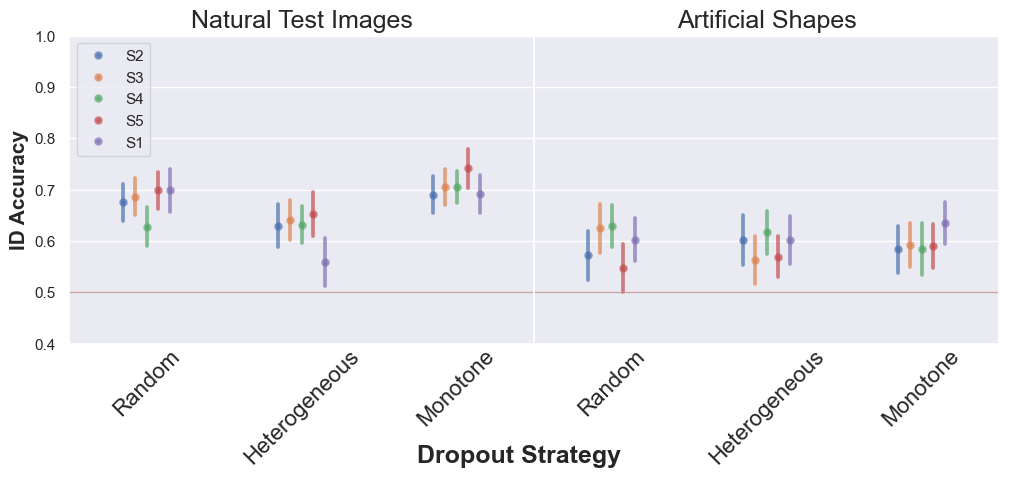
\includegraphics[width=1\textwidth]{plots/dropout_discussion_translator_id_acc_vdvae.png}
   \caption[VDVAE translator Results for monotone vs.\ heterogeneous training images]{VDVAE translator Results for monotone vs.\ heterogeneous training images. The identification accuracy of the VDVAE translator is displayed for a different samples of the training data: a random subset, a heterogeneous subset, a monotone subset and the full training data. The results are shown for both the natural test images and the artificial shapes. The data is shown for each subject, the error bars are computed as the standard error across all test samples.}\label{fig:dropout_discussion_translator_id_acc_vdvae}
 \end{figure}
 
 \begin{figure}[H]
   \centering
   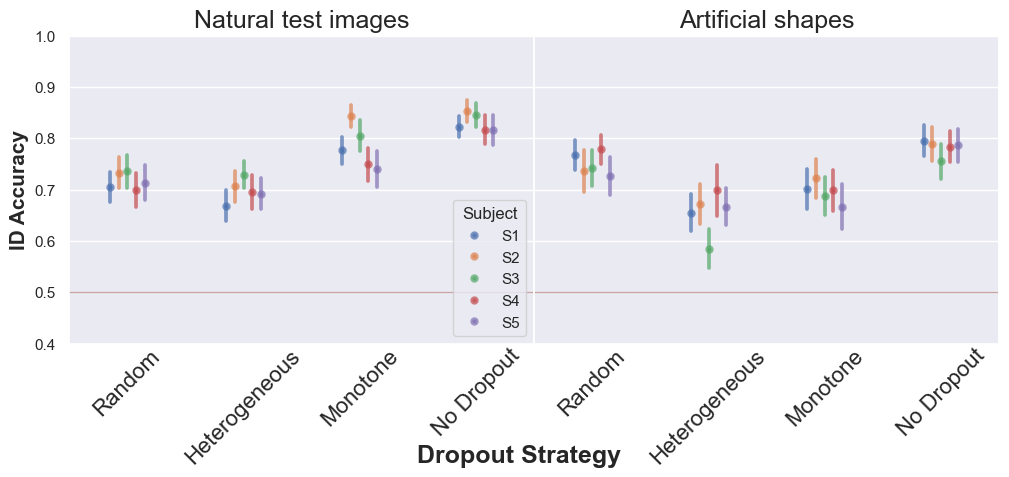
\includegraphics[width=1\textwidth]{plots/dropout_discussion_translator_id_acc_icnn.png}
   \caption[iCNN translator Results for monotone vs.\ heterogeneous training images]{iCNN translator Results for monotone vs.\ heterogeneous training images. The identification accuracy of the iCNN translator is displayed for a different samples of the training data: a random subset, a heterogeneous subset, a monotone subset and the full training data. The results are shown for both the natural test images and the artificial shapes. The data is shown for each subject, the error bars are computed as the standard error across all test samples.}\label{fig:dropout_discussion_translator_id_acc_icnn}
 \end{figure}
 
 \begin{figure}[H]
   \centering
   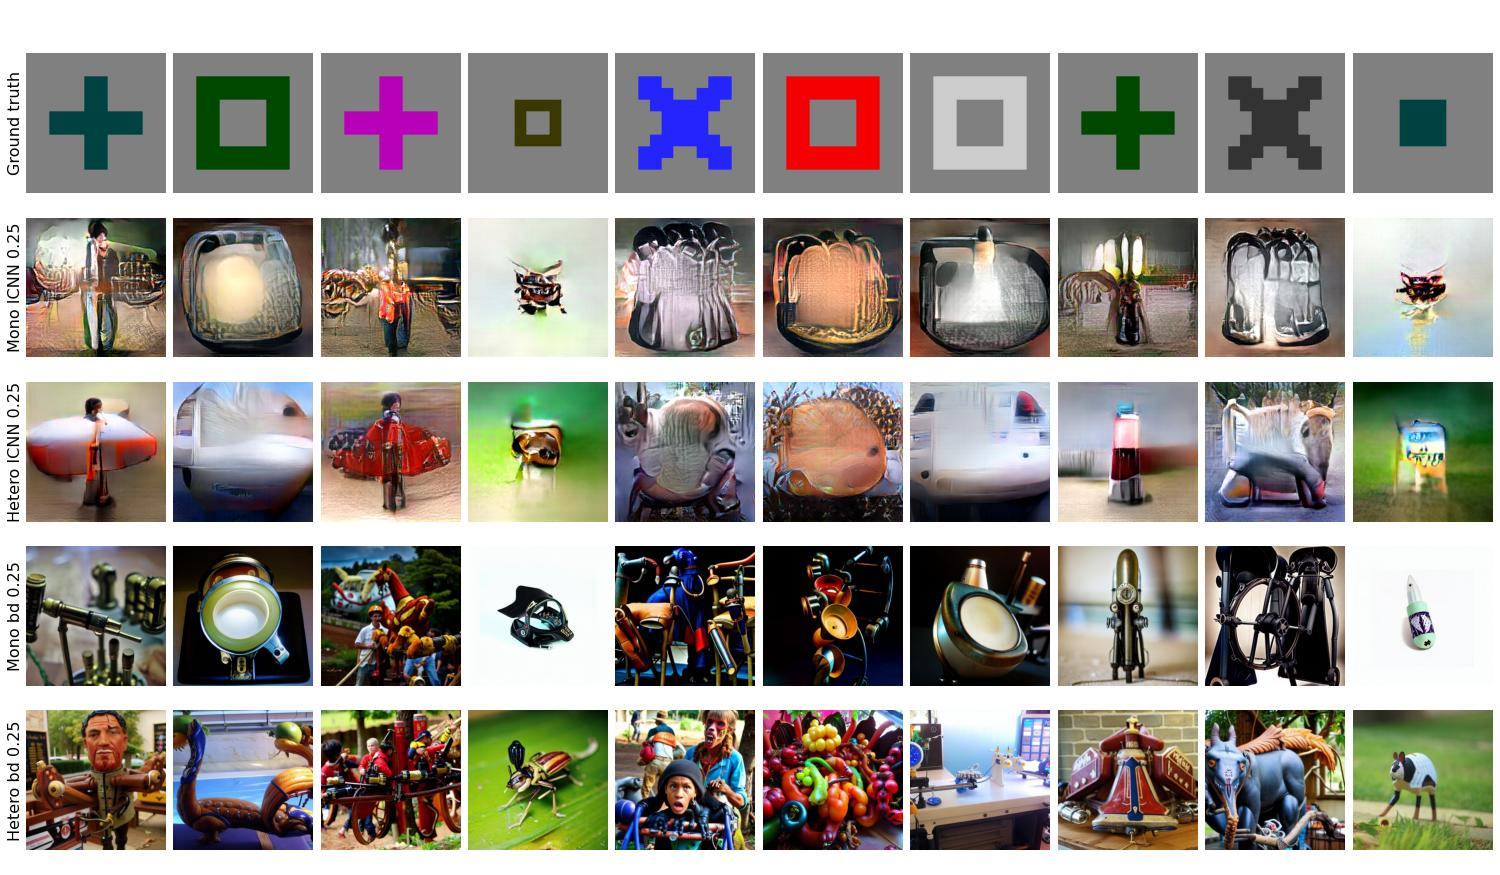
\includegraphics[width=1\textwidth]{plots/dropout_discussion_art.JPEG}
   \caption[Reconstructed images with monotonous and heterogeneous training data on artificial shapes]{Qualitative Results for monotone vs.\ heterogeneous training images on artificial shapes. The top row depicts the ground truth image. Each following row depicts the reconstruction where the translator was trained using the dropout strategy and algorithm (note: bd stands for Brain-Diffuser) defined on the left side.}\label{fig:dropout_discussion_art}
 \end{figure}


\section{Ai Captions}

\begin{figure}[H]
   \centering
   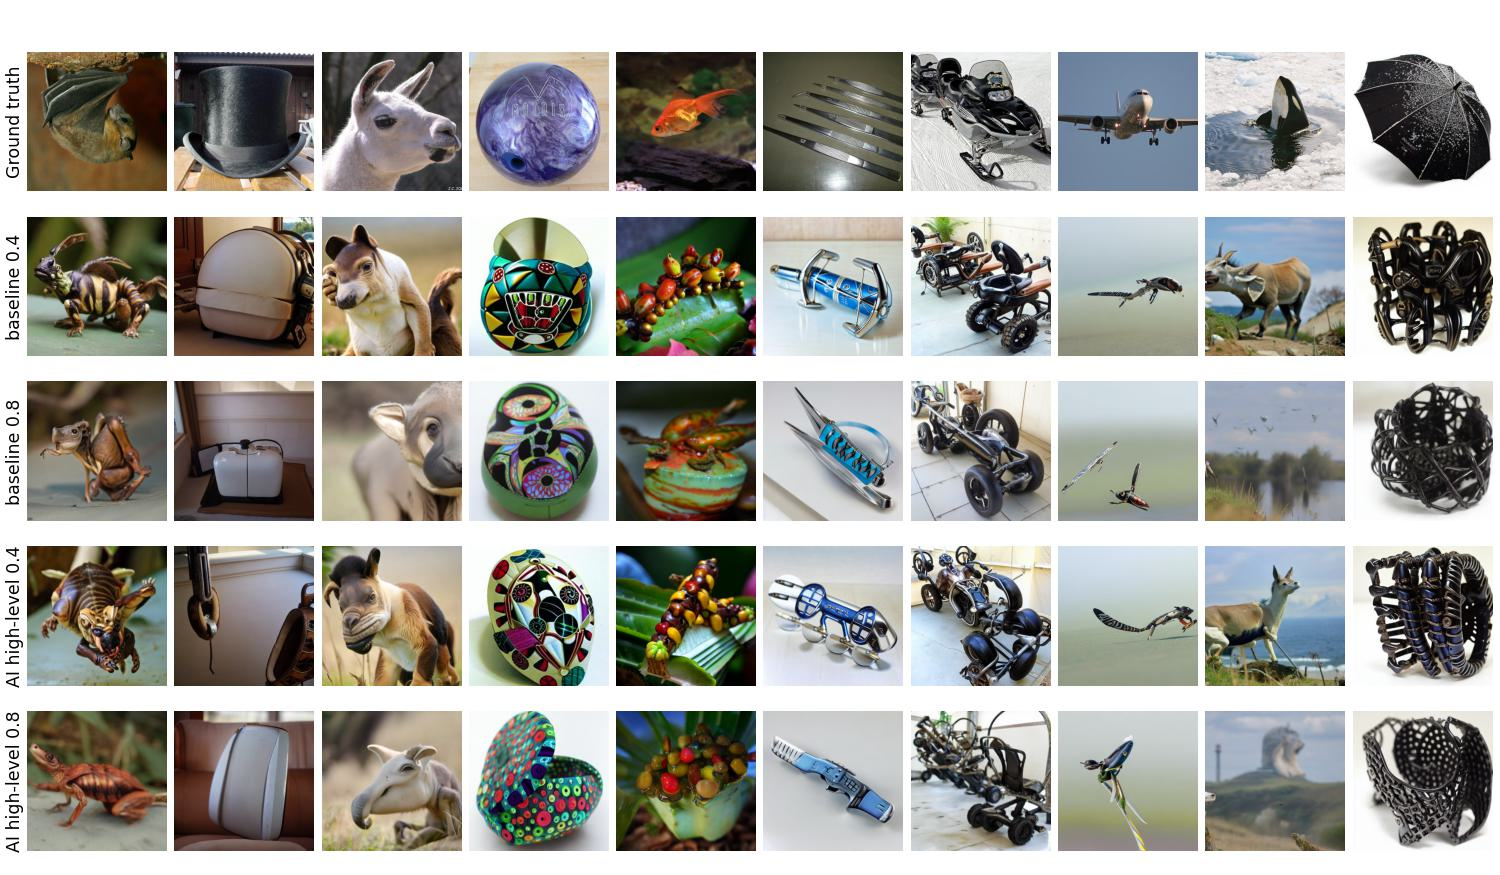
\includegraphics[width=1\textwidth]{plots/aicap_qual_test_highlevel_appendix.JPEG}
   \caption[Experiment 2: Reconstructed images for Brain-Diffuser on natural test images with high-level captions]{Qualitative Results for the high-level AI captions on natural test images. The top row depicts the ground truth image. Each following row depicts the reconstruction where the CLIP Text translator was trained with either human generated captions (baseline) or AI generated low-level captions. Additionally, the results are displayed for the mixing parameter 0.4 and 0.8.}\label{fig:aicap_qual_test_highlevel_appendix}
\end{figure}

\begin{figure}[H]
   \centering
   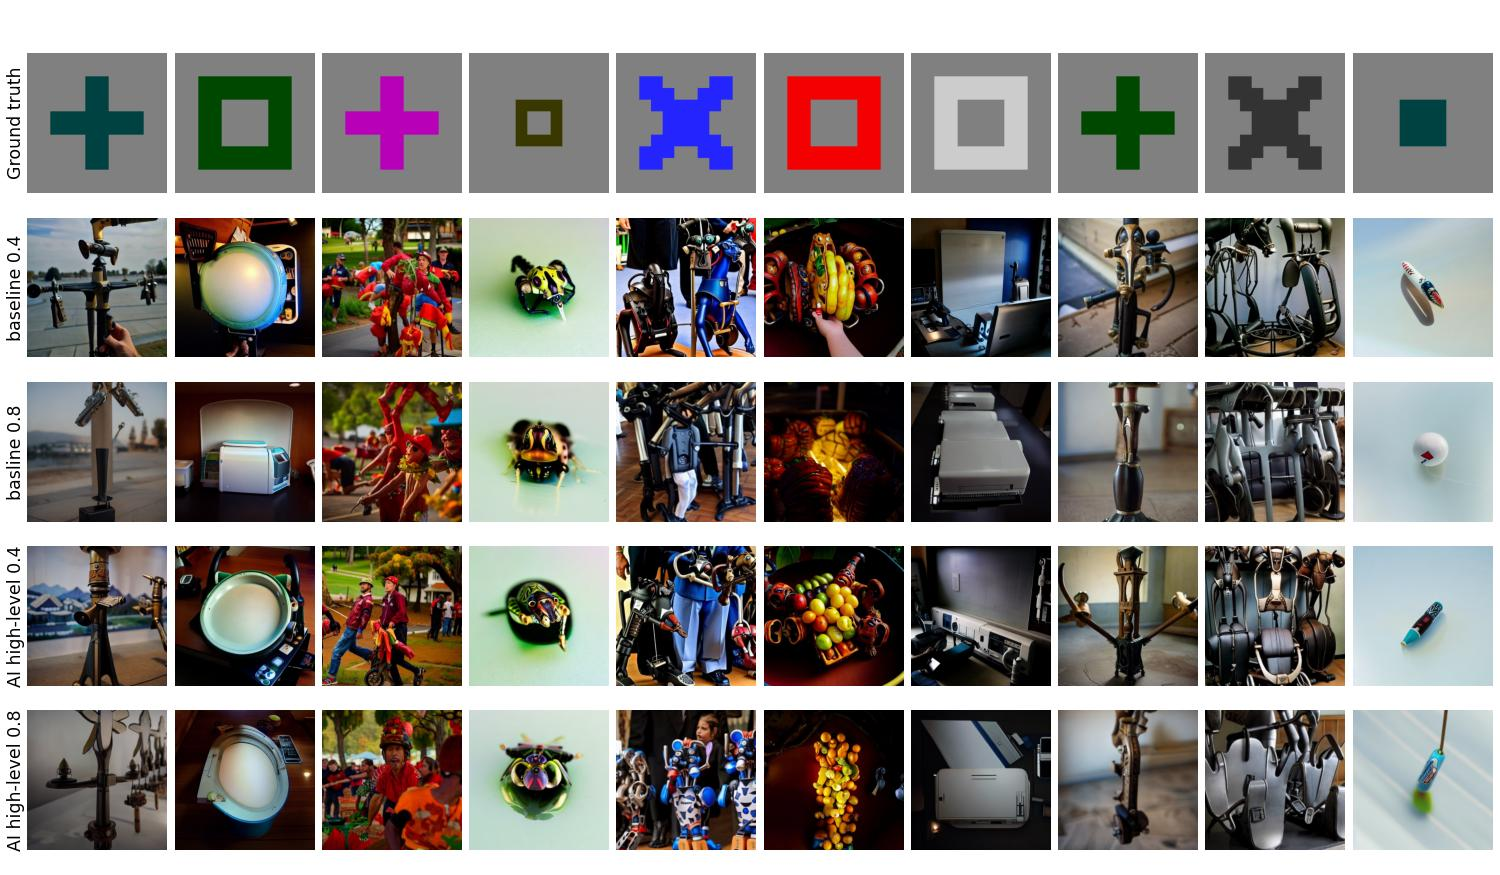
\includegraphics[width=1\textwidth]{plots/aicap_qual_art_highlevel_appendix.JPEG}
   \caption[Experiment 2: Reconstructed images for Brain-Diffuser on artificial shapes with high-level captions]{Qualitative Results for the high-level AI captions on artificial shapes. The top row depicts the ground truth image. Each following row depicts the reconstruction where the CLIP Text translator was trained with either human generated captions (baseline) or AI generated low-level captions. Additionally, the results are displayed for the mixing parameter 0.4 and 0.8.}\label{fig:aicap_qual_art_highlevel_appendix}
\end{figure}


\begin{figure}[H]
   \centering
   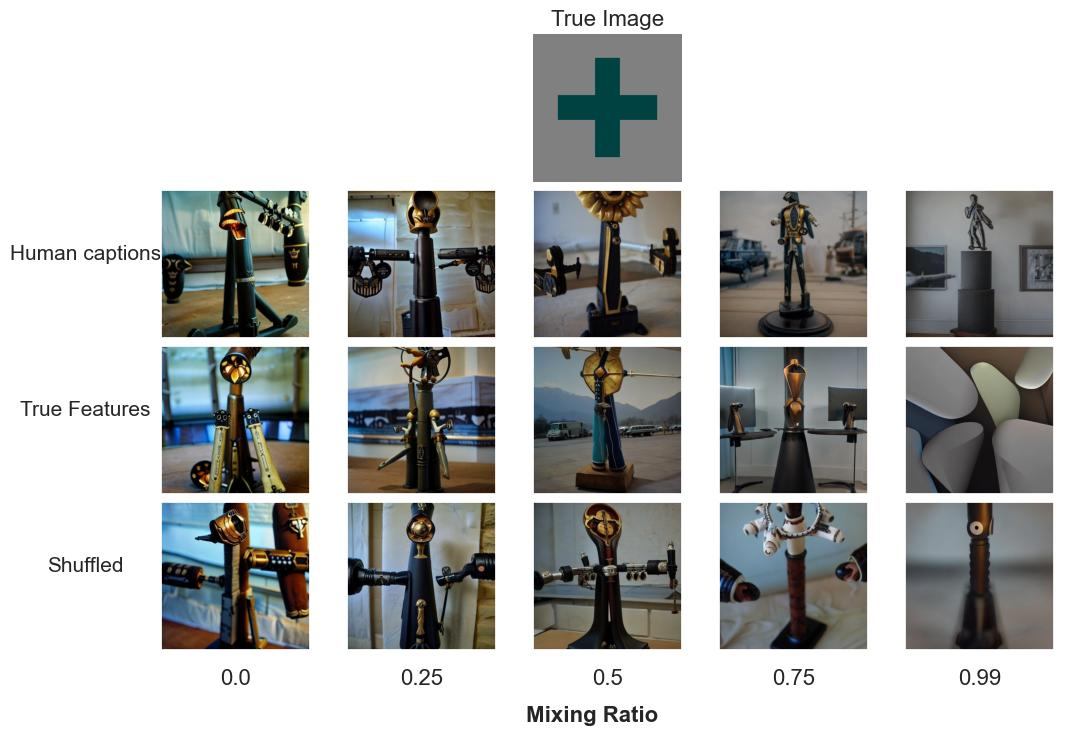
\includegraphics[width=1\textwidth]{plots/aicap_reconstruction_evolution_art_0.JPEG}
   \caption[Influence of the mixing ratio on artificial shapes]{Qualitative influence of different mixing ratio on artificial shapes. For three different CLIP Text features (predicted from human captions, predicted from shuffled captions and true features), the reconstruction is shown for varying levels of the mixing ratio in the diffusion process.}\label{fig:aicap_reconstruction_evolution_art_0}
\end{figure}

\begin{figure}[H]
   \centering
   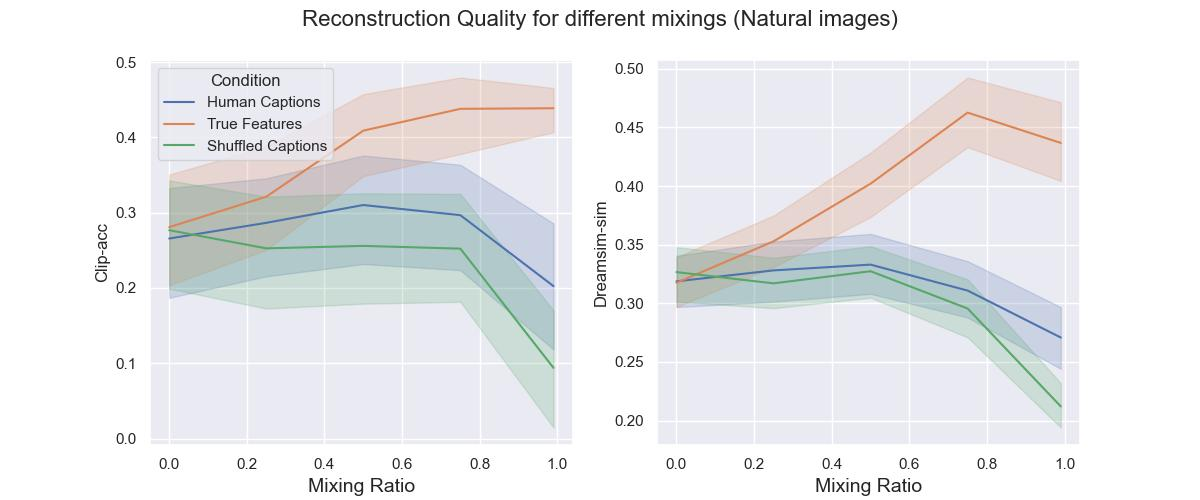
\includegraphics[width=1\textwidth]{plots/aicap_reconstruction_quant_evolution_test.JPEG}
   \caption[Quantitative influence of different mixing ratios on natural test images]{Quantitative influence of different mixing ratios on natural test images. The CLIP-accuracy and dreamsim of the reconstructions on natural test images are shown for an increasing mixing ratio.}\label{fig:aicap_reconstruction_quant_evolution_test}
\end{figure}

\begin{figure}[H]
   \centering
   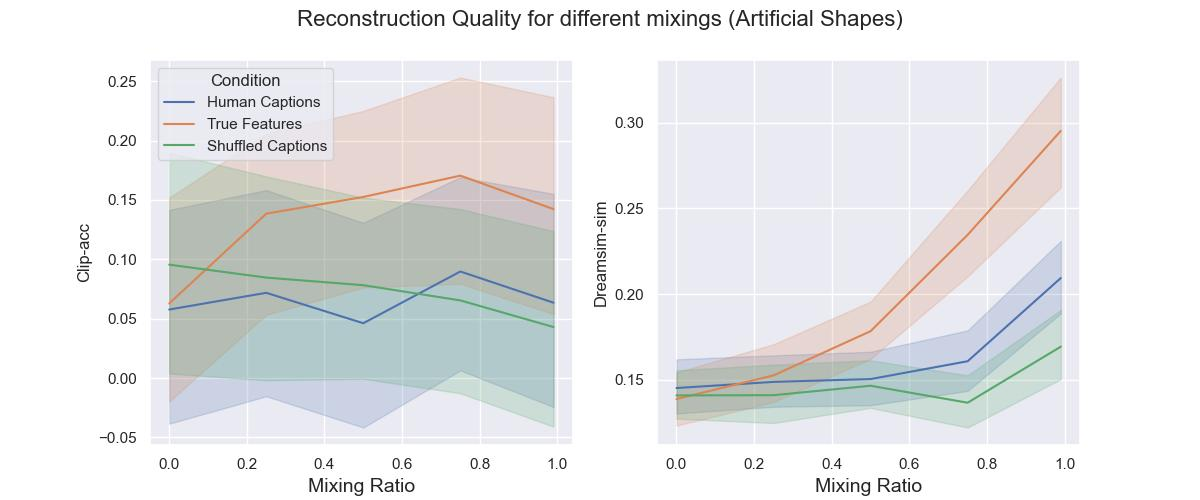
\includegraphics[width=1\textwidth]{plots/aicap_reconstruction_quant_evolution_art.JPEG}
   \caption[Quantitative influence of different mixing ratios on artificial shapes]{Quantitative influence of different mixing ratios on artificial shapes. The CLIP-accuracy and dreamsim of the reconstructions on artificial shapes are shown for an increasing mixing ratio.}\label{fig:aicap_reconstruction_quant_evolution_art}
\end{figure}

\section{Perturbations}
\begin{figure}[H]
    \centering
    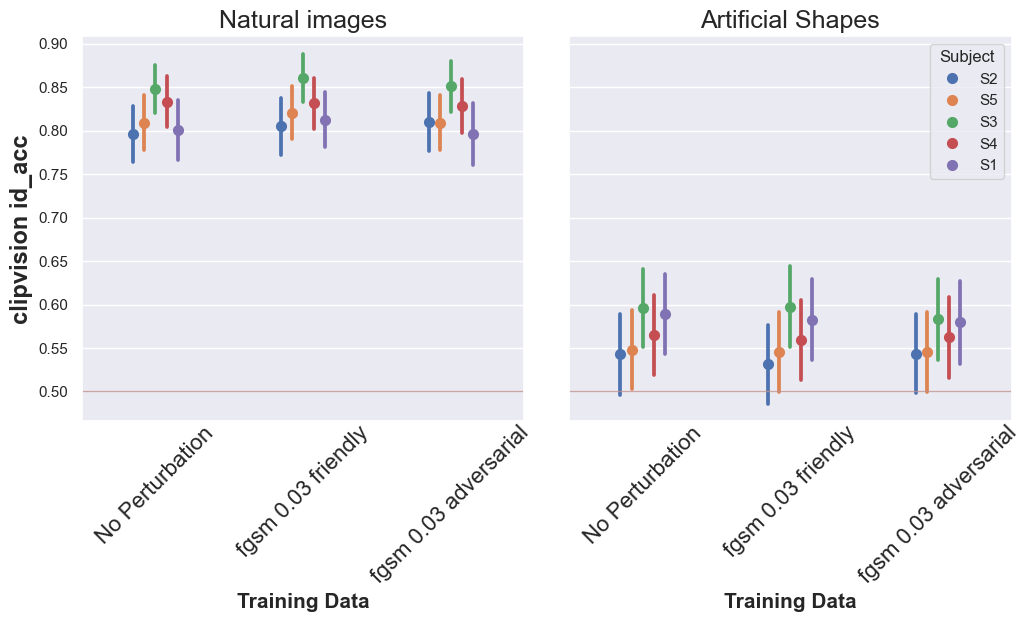
\includegraphics[width=1\textwidth]{plots/advpert_translator_fgsm_0.03.png}
    \caption[Experiment 3: Translator performance with FGSM]{Translator performance for friendly and adversarial perturbation with the FGSM algorithm. The CLIP Vision identification accuracy is displayed for each subject with either no perturbation, friendly perturbation or adversarial perturbation. The results are displayed both for the natural test images and the artificial shapes. The error bars are computed as the standard errors across all test samples.}\label{fig:advpert_translator_fgsm_0}
\end{figure}

\begin{figure}[H]
    \centering
    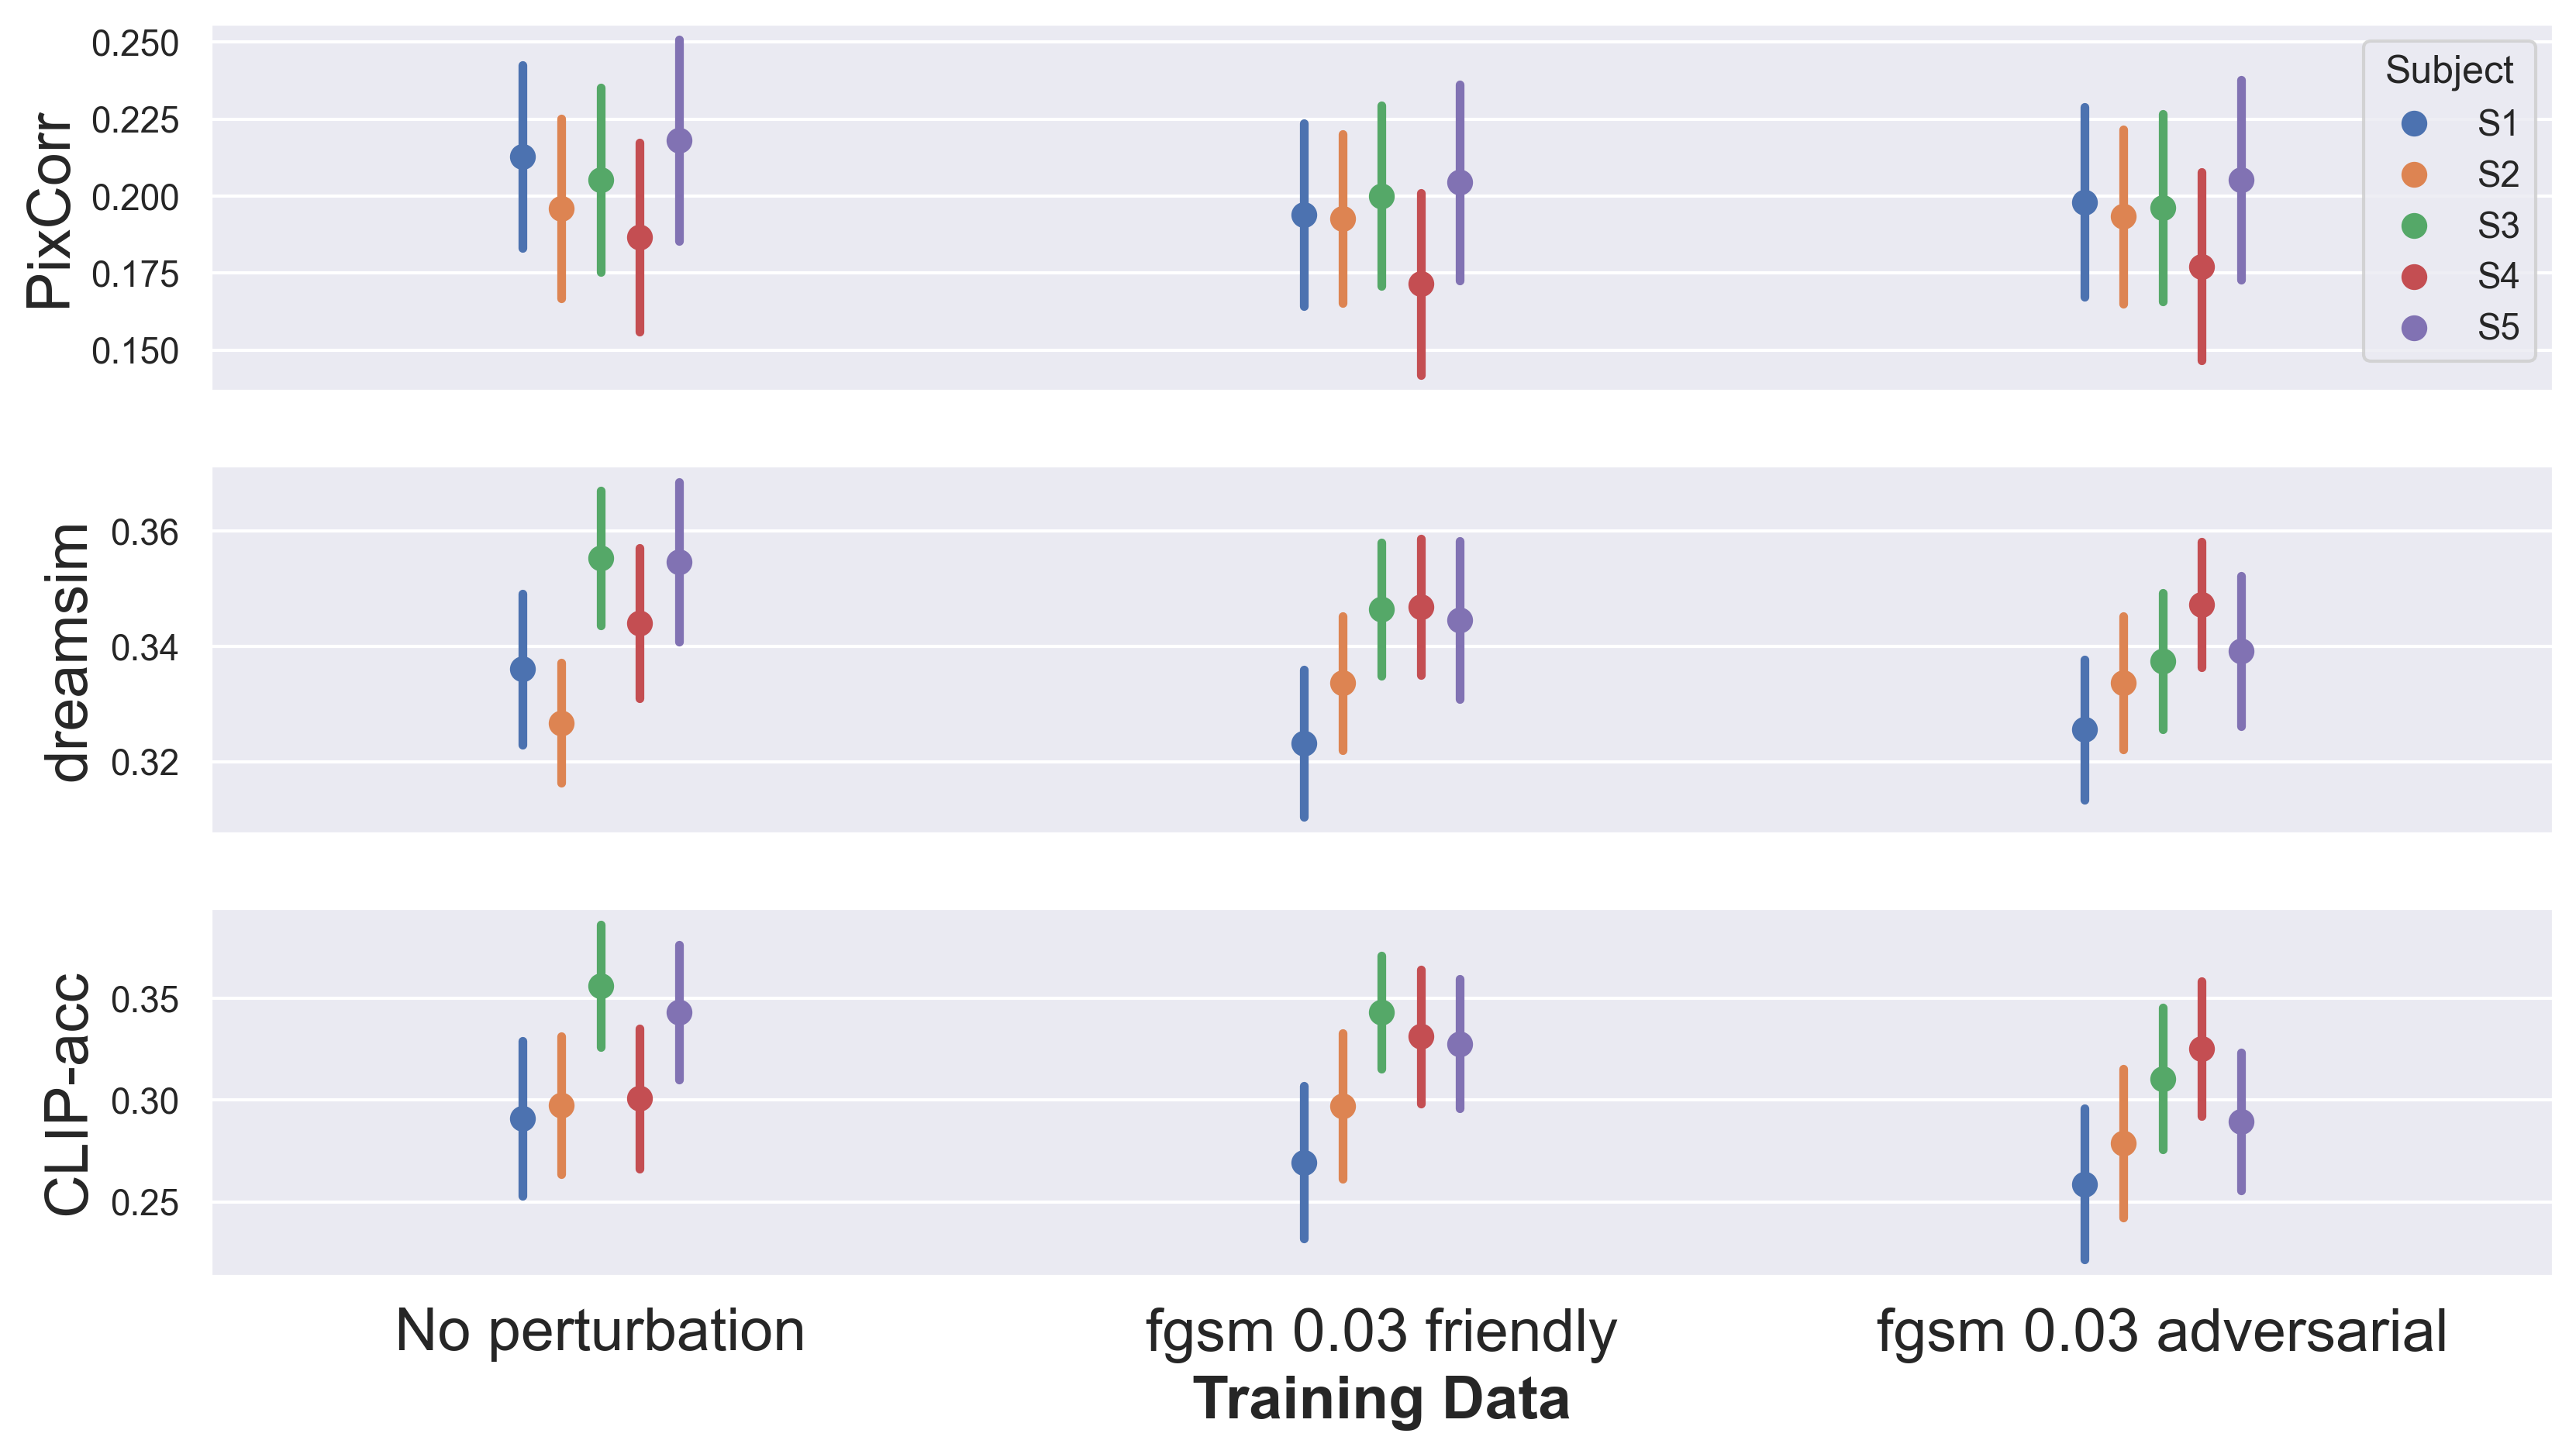
\includegraphics[width=1\textwidth]{plots/advpert_reconstruction_test_fgsm_0.03.png}
    \caption[Experiment 3: Reconstruction performance on natural test images with FGSM]{Reconstruction performance on natural test images. The three reconstruction performance criteria (PixelCorrelation, dreamsim and CLIP-accuracy) are displayed for the baseline training dataset and the perturbed dataset with either friendly or adversarial perturbations using the FGSM 0.03 algorithm. The data is shown for each subject and the error bars are computed as the standard errors across all test samples.}\label{fig:advpert_reconstruction_test_fgsm_0.03}
\end{figure}

\begin{figure}[H]
    \centering
    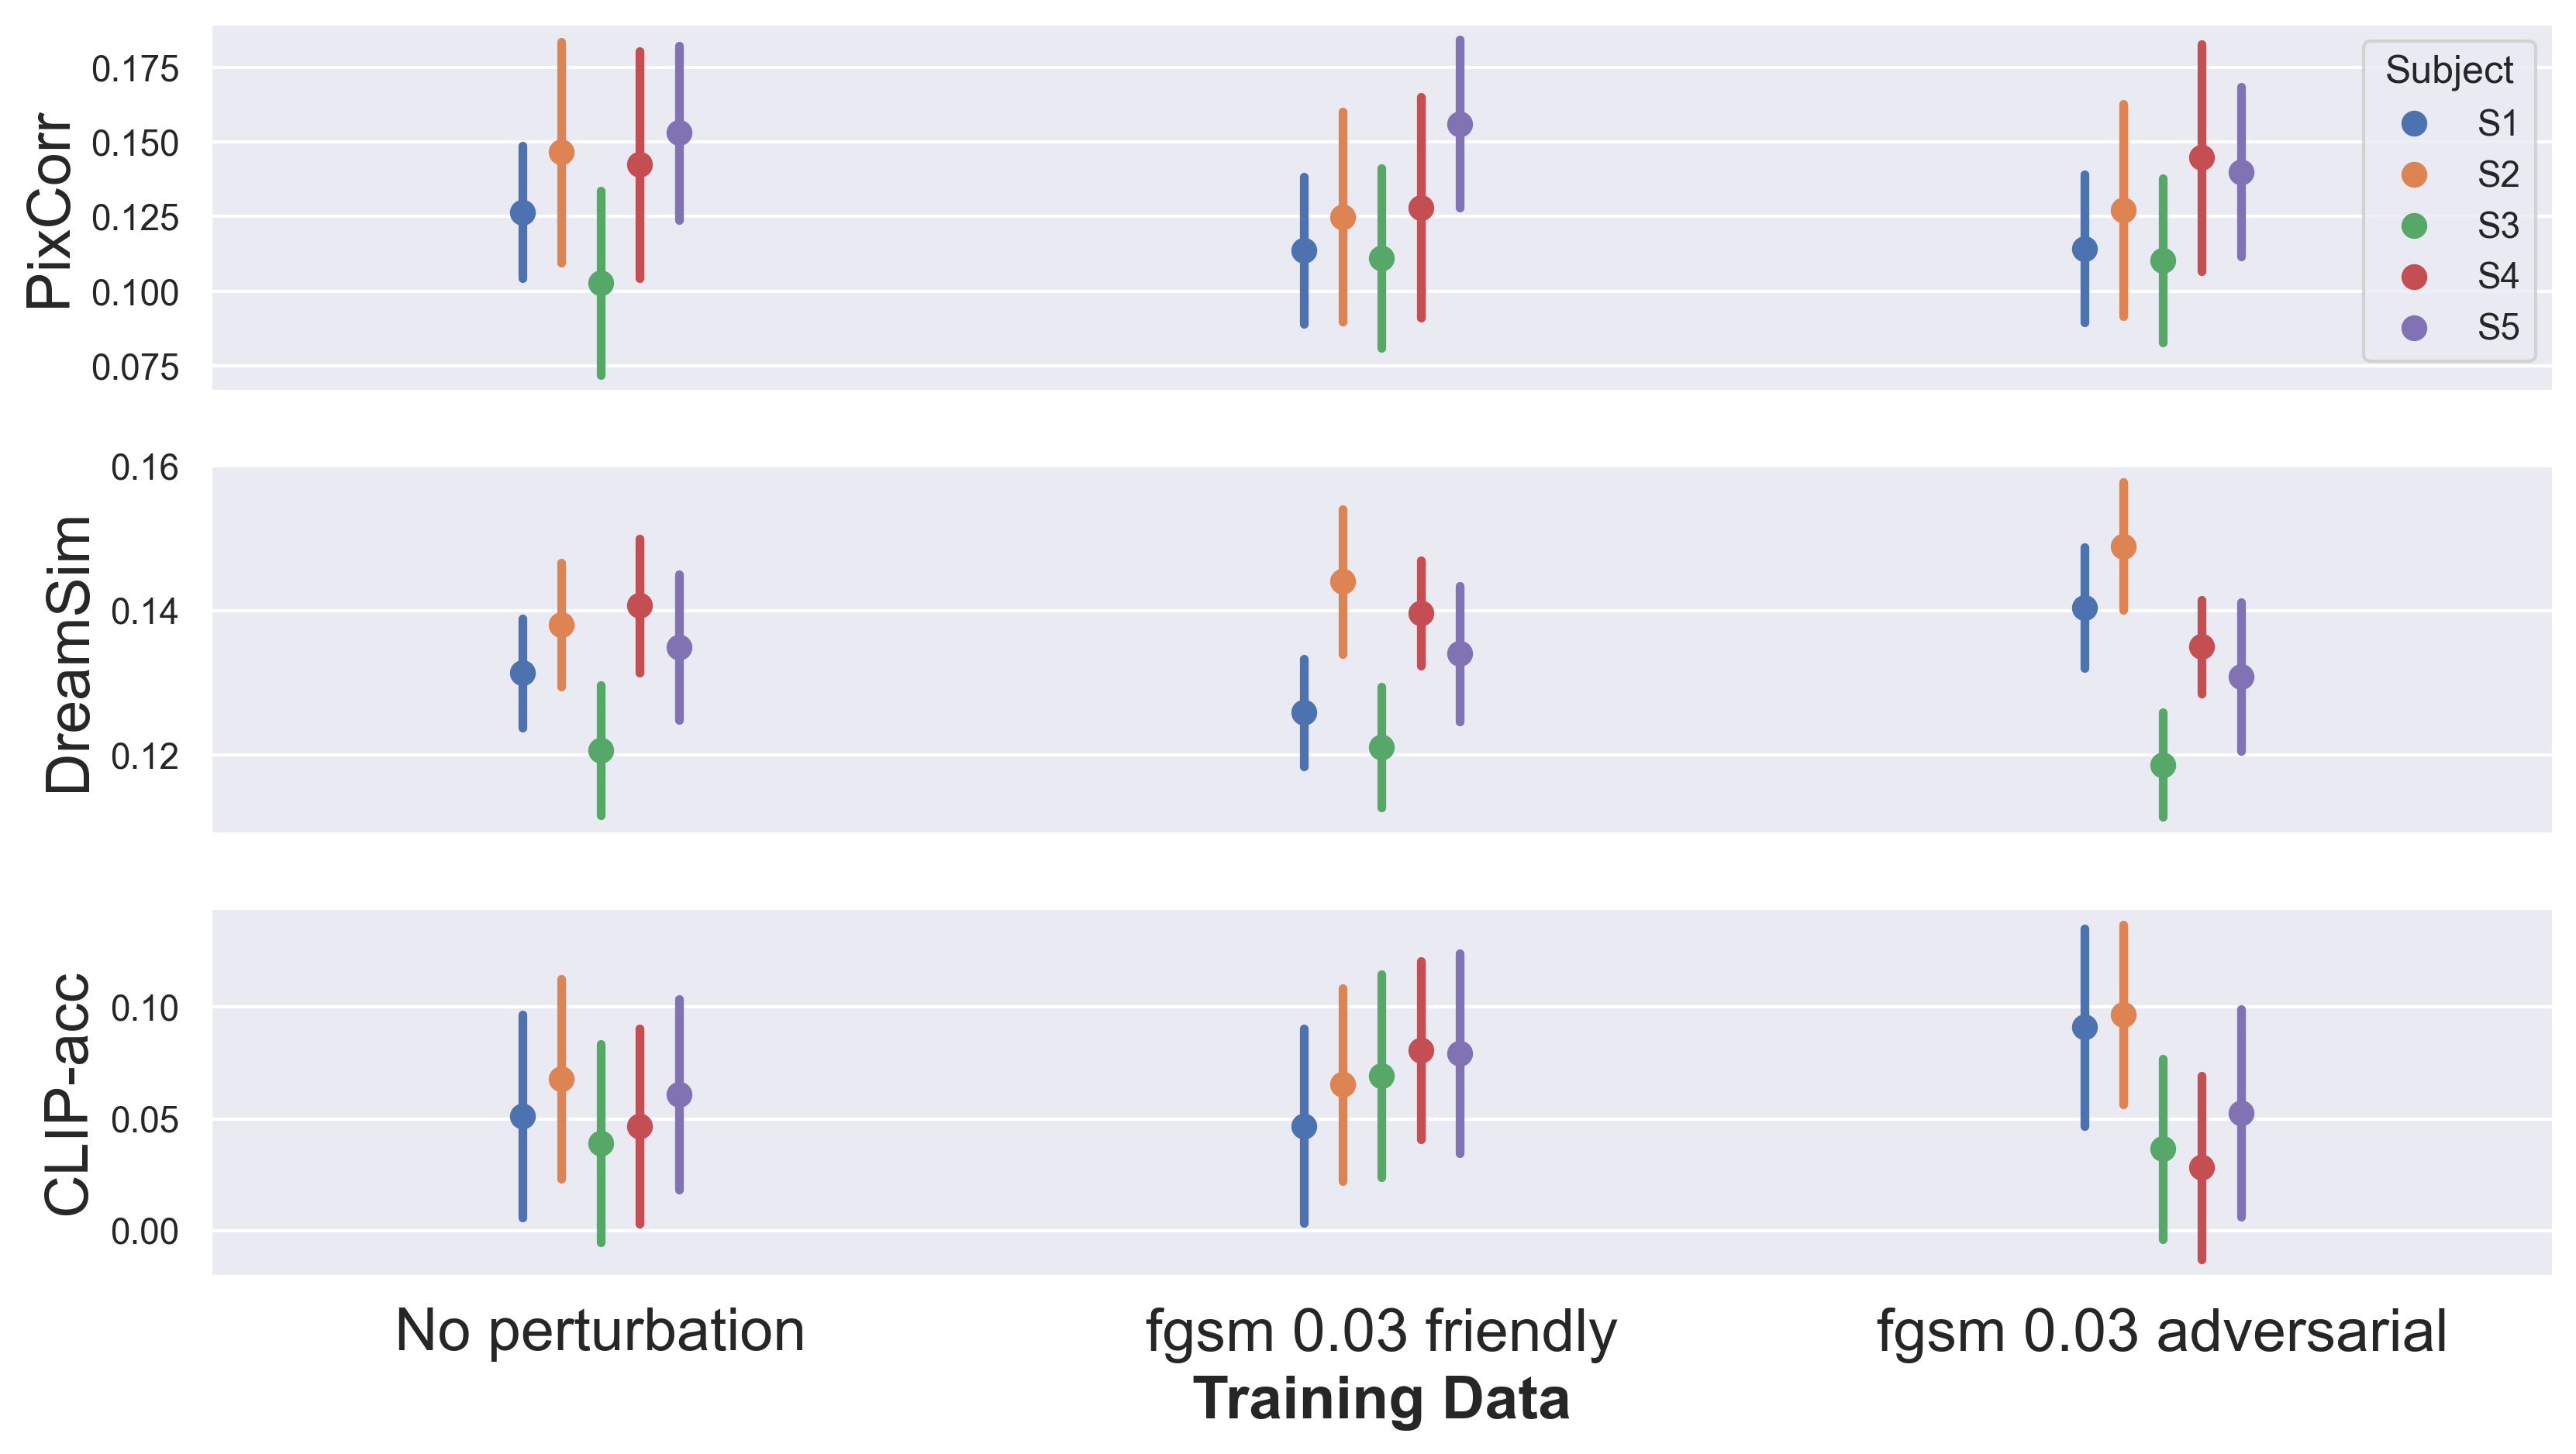
\includegraphics[width=1\textwidth]{plots/advpert_reconstruction_art_fgsm_0.03.png}
    \caption[Experiment 3: Reconstruction performance on artificial shapes with FGSM]{Reconstruction performance on artificial shapes. The three reconstruction performance criteria (PixelCorrelation, dreamsim and CLIP-accuracy) are displayed for the baseline training dataset and the perturbed dataset with either friendly or adversarial perturbations using the FGSM 0.03 algorithm. The data is shown for each subject and the error bars are computed as the standard errors across all test samples.}\label{fig:advpert_reconstruction_art_fgsm_0.03}
\end{figure}

\begin{figure}[H]
   \centering
   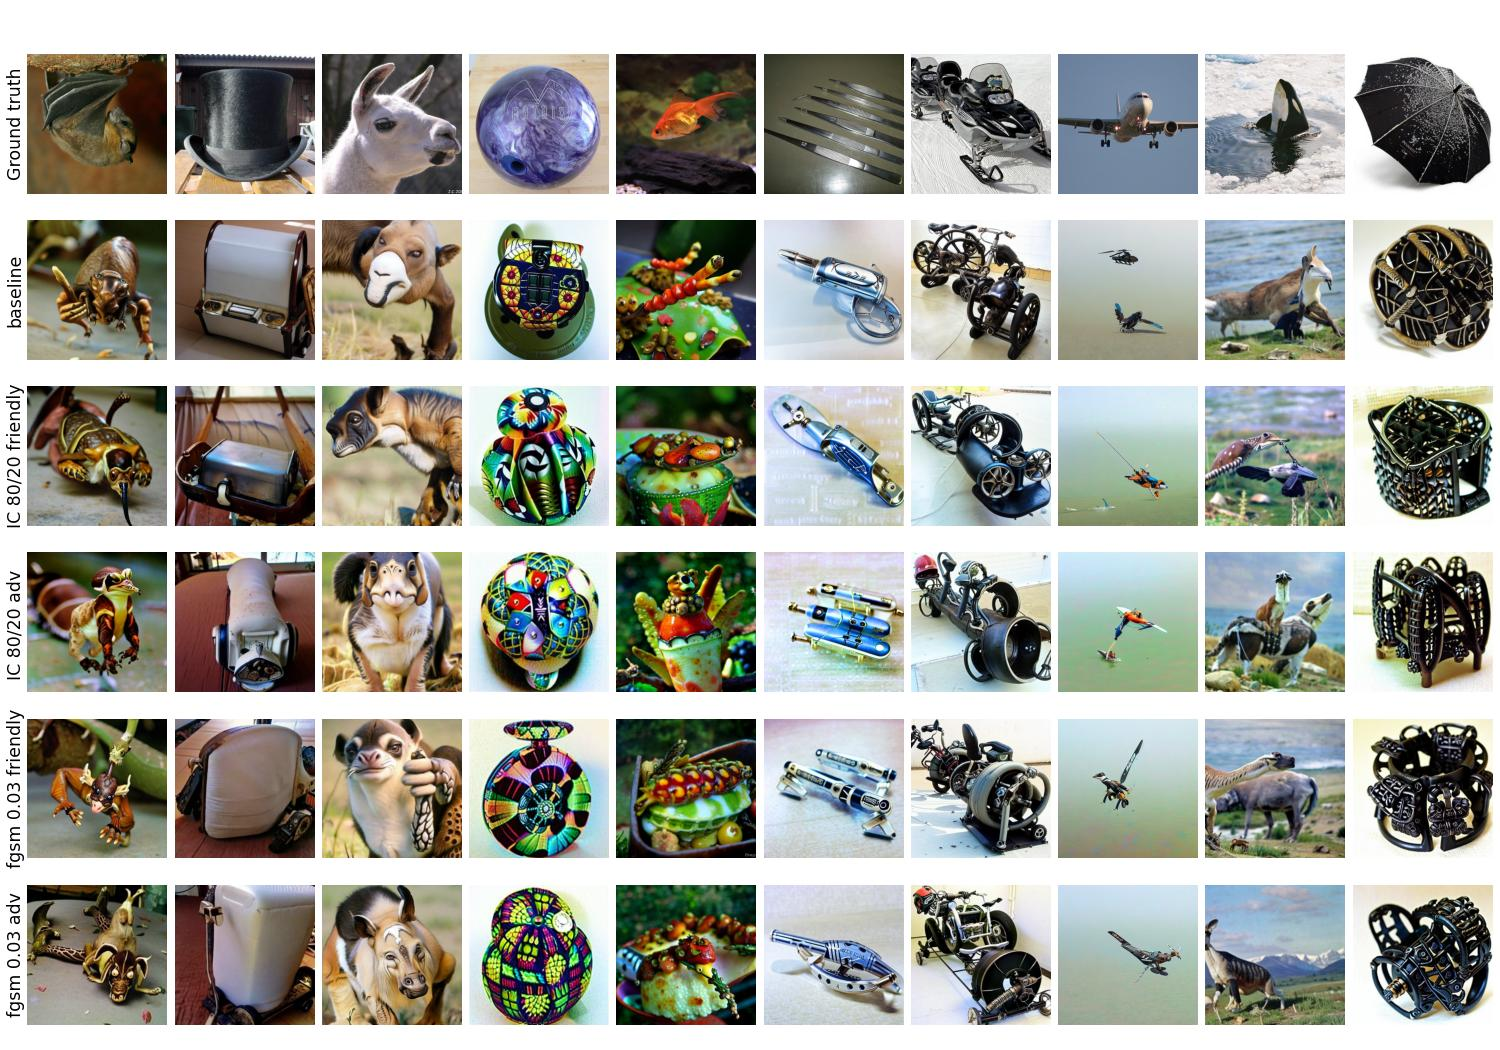
\includegraphics[width=1\textwidth]{plots/advpert_qual_test.JPEG}
   \caption[Experiment 3: Reconstructed images on natural test images for different perturbations]{Qualitative Results for the different perturbations on natural test images. The top row depicts the ground truth image. Each following row depicts the reconstruction where the CLIP Vision translator was trained with perturbated images with either friendly or adversarial (adv) perturbations using the IC80/20 or FGSM 0.03 algorithm.}\label{fig:advpert_qual_test}
\end{figure}

\begin{figure}[H]
   \centering
   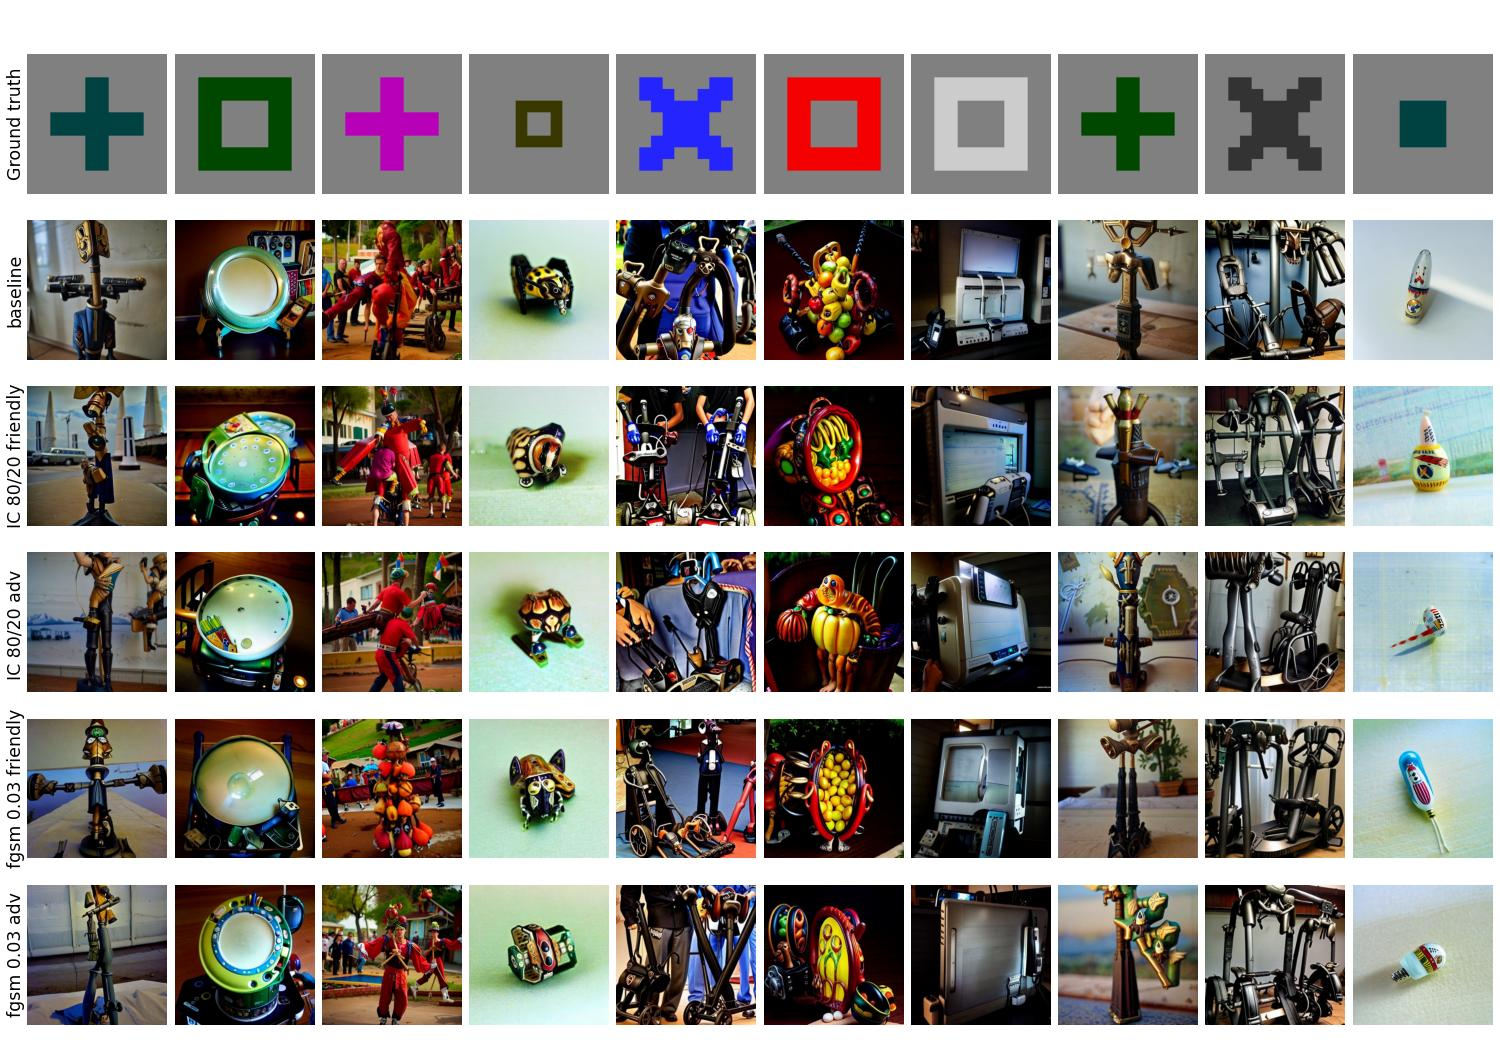
\includegraphics[width=1\textwidth]{plots/advpert_qual_art.JPEG}
   \caption[Experiment 3: Reconstructed images on artificial shapes for different perturbations]{Qualitative Results for the different perturbations on artificial shapes. The top row depicts the ground truth image. Each following row depicts the reconstruction where the CLIP Vision translator was trained with perturbated images with either friendly or adversarial (adv) perturbations using the IC80/20 or FGSM 0.03 algorithm.}\label{fig:advpert_qual_art}
\end{figure}

